\documentclass[11pt]{article}

\usepackage[a4paper,margin=2.4cm]{geometry}
\usepackage[T1]{fontenc}
\usepackage[utf8]{inputenc}
\usepackage{graphicx}
\usepackage{subcaption}
\usepackage{booktabs}
\usepackage{amsmath}
\usepackage{amssymb}
\usepackage{siunitx}
\usepackage{xcolor}
\usepackage{listings}
\usepackage{comment}
\usepackage{tabularx}
\newcolumntype{Y}{>{\raggedright\arraybackslash}X}
\usepackage[hidelinks]{hyperref}
\usepackage{caption}
\captionsetup{font=small}
\newcommand{\authorline}[1]{\noindent\textit{Author: #1}\par\medskip}
\setlength{\parindent}{0pt}

% Figures exported by the experiments are stored in the report/imgs/ folder.
\graphicspath{{imgs/}}

\newcommand{\code}[1]{\texttt{#1}}
\newcommand{\todo}[1]{\textcolor{red}{[TODO: #1]}}

\title{\textbf{Reinforcement Learning for Bomberman}}
\author{Luis David Maco Cangalaya \and Diana Krasnokutskaya \and Daniela Ardila Porras}
\date{Machine Learning Essentials -- Summer Semester 2026}

\begin{document}
\maketitle

% ============================================================
\section{Introduction}
\label{sec:intro}
% ============================================================

\authorline{Diana Krasnokutskaya}

Bomberman is a simple game with a surprisingly hard decision problem underneath. In the
version used for this project, four agents move on a $17\times17$ grid of walls, crates and
free tiles for at most 400 steps. In each step an agent picks one of six actions: four
moves, waiting, or dropping a bomb. A bomb explodes after four steps and destroys everything
within three tiles in a straight line until a wall stops the blast. Crates can hide coins.
A coin is worth one point, and blowing up an opponent is worth five. The agent has
0.5\,seconds of CPU time per step to decide what to do. Our goal was to train an agent with
reinforcement learning (RL) that plays this game as well as possible, and in particular one
that beats the provided \code{rule\_based\_agent} on the \code{classic} board. 

\hspace{1cm}

We worked through four tasks of increasing difficulty:
\begin{itemize}
\item[(1)] collecting coins on an empty board
\item[(2)] destroying crates and finding hidden coins
without killing oneself
\item[(3)] hunting the provided \code{peaceful\_agent} and
\code{coin\_collector\_agent}
\item[(4)] holding one's own against the full-strength
\code{rule\_based\_agent}. 
\end{itemize}
Tasks 1--3 serve as stepping stones and debugging stages. Task~4 is
the criterion the tournament actually rewards.

\hspace{1cm}

The task is small and cheap to simulate, but still includes many of the challenges that make reinforcement learning difficult in practice.
\begin{itemize}
  \item \textbf{Delayed and sparse credit.} Rewards are rare. An agent that walks into its
        own blast dies four steps after the decision that actually killed it, and the step
        that traps an opponent happens well before the opponent dies. Credit has to travel
        back through several steps.
  \item \textbf{Safety-critical actions.} One wrong bomb ends the round. For every agent we
        trained, a large share of all losses came from suicides rather than from opponents.
  \item \textbf{A non-stationary, multi-agent environment.} From task 3 on, other agents
        drop bombs and compete for the same coins, so a safe state can become deadly
        because of someone else's decision.
  \item \textbf{A large state space.} Tabular Q-learning over raw boards is impossible. We
        either design a compact feature representation by hand or let a neural network
        learn one.
  \item \textbf{Limited compute and time.} Three weeks, one CPU thread per agent in the
        tournament.
\end{itemize}

\newpage

\begin{comment}
We developed two structurally different agents:
\begin{enumerate}
  \item \textbf{\code{q\_agent}}, a linear Q-learning agent over 34 hand-engineered features
        (walkability, danger countdowns, BFS directions to coins, crates, safe tiles and
        opponents, and a few bomb-specific indicators). It uses an action mask that removes
        illegal and provably suicidal actions, and a hand-designed set of auxiliary rewards.
  \item \textbf{\code{dqn\_agent}}, a Double Deep Q-Network with a target network and
        experience replay. It reads a six-channel image of the board (walls, crates, self,
        others, coins, danger) through a convolutional encoder and learns its own features.
        It deliberately contains no path-finding or danger heuristics in its state encoding.
\end{enumerate}

The two agents answer the central question of this report from opposite sides: with a
fixed time budget, is it better to put domain knowledge into hand-crafted features or to
let a network learn the representation?
\end{comment}

We developed two structurally different agents, \textbf{\code{q\_agent}} and \textbf{\code{dqn\_agent}}, which approach the learning problem in different ways. While \textbf{\code{q\_agent}} relies on manually designed representations incorporating domain knowledge, \textbf{\code{dqn\_agent}} learns its representation directly from the game state. This allows us to investigate the central question of this report: under a fixed time budget, how does the use of domain knowledge compare to learning representations directly from the environment?

%\authorline{Diana Krasnokutskaya}

% ============================================================
\section{Background}
\label{sec:background}
\authorline{Daniela Ardila}
% ============================================================
\subsection{Bomberman as a Markov decision process}
\label{sec:bg-mdp}
 
Building on the rules summarized in Section~\ref{sec:intro}, we describe here the
details of the game that are relevant to decide which method is the best approach, and
state the game in the notation of the lecture~\cite{koethe2026mle}.
An explosion stays lethal for one more step after the detonation, and each
agent can only have one bomb at a time. Only the wall layout is fixed. Crates, coins and
start corners are re-randomized every round, and on the \code{classic} board all nine
coins start hidden under crates. So the agent cannot memorize a board, but has to
generalize to new layouts. Since almost everything is visible and the countdowns of all
bombs and explosions are part of the game state, we use the lecture's simplification to
a fully observed Markov decision process (MDP), $o_t = s_t$:
\begin{itemize}\setlength{\itemsep}{1pt}
  \item \textbf{Time:} one round is one episode with steps $t = 1,\dots,T$, where
        $T \le 400$. In training mode the round ends when our agent dies, so death is a
        terminal state.
  \item \textbf{States} $s_t$: the \code{game\_state}, with the field (walls, crates,
        free tiles), the bombs with their countdowns, the explosion map, the visible
        coins, and position, score and bomb availability of our agent (\code{self}) and
        of the opponents still alive (\code{others}).
  \item \textbf{Actions} $a_t \in A = \{\mathrm{UP}, \mathrm{DOWN}, \mathrm{LEFT},
        \mathrm{RIGHT}, \mathrm{WAIT}, \mathrm{BOMB}\}$.
  \item \textbf{Rewards} $r_{t+1}$: the official reward is $+1$ per coin, $+5$ per kill
        and $0$ otherwise, so it is zero in most steps. Therefore we train with a shaped
        reward $\hat r_{t+1}$ (Section~\ref{sec:methods}), which can bias the policy
        unless the extra rewards have the form of a potential $\psi$,
        $\hat r_{t+1} = r_{t+1} + \gamma\,\psi(s_{t+1}) - \psi(s_t)$, with the discount
        factor $\gamma$ of Section~\ref{sec:bg-value}~\cite{koethe2026mle,ng1999}.
  \item \textbf{World probability} $p^*(s_{t+1}, r_{t+1} \mid s_t, a_t)$: the
        deterministic game engine together with the random order in which the actions
        are executed, the hidden coins and the opponents' actions. Since the opponents'
        policies are unknown, $p^*$ is unknown too, so we use model-free RL, which learns
        only from observed transitions~\cite{koethe2026mle}.
  \item \textbf{Policy} $\pi(a_t \mid s_t)$: the probability that our agent plays $a_t$
        in $s_t$; the goal is the optimal policy $\pi^*$.
  \item \textbf{Training set} (TS): the observed transitions
        $(s_t, a_t, r_{t+1}, s_{t+1})$.
\end{itemize}
The state space is huge: 164 of the 176 free tiles can hold a crate, so there are already
$2^{164} \approx 2\cdot10^{49}$ crate layouts, and a table with one value per
state-action pair is impossible.

\subsection{Value functions and Q-learning}
\label{sec:bg-value}
 
To find the best policy of an MDP, we need value functions. We first introduce them and
then show how they are learned from the TS. Usually the discounted return is used, which
weights rewards further in the future less. The agent maximizes this return, and the
optimal policy maximizes its expectation~\cite{koethe2026mle,sutton2018}:
\begin{equation}
  g_t = \sum_{t'=t+1}^{T+1} \gamma^{\,t'-(t+1)}\, r_{t'}, \quad \gamma \in (0,1],
  \qquad
  \pi^* = \operatorname*{arg\,max}_{\pi}\; \mathbb{E}_{p^*,\pi}\bigl[g_1\bigr].
\end{equation}
The value function $V_\pi(s)$ is the expected return when we start in $s$ and follow
$\pi$, and the action-value function $Q_\pi(s,a)$ the expected return when we play $a$ in
$s$ and follow $\pi$ afterwards:
\begin{equation}
  Q_\pi(s,a) = \mathbb{E}_{s',r\sim p^*}\bigl[r + \gamma\, V_\pi(s')\bigr],
  \qquad
  V_\pi(s) = \mathbb{E}_{a\sim\pi(a\mid s)}\bigl[Q_\pi(s,a)\bigr].
\end{equation}
If $p^*$ were known, the resulting Bellman equation could be solved by value iteration.
With $Q$, $p^*$ is not needed: the best action is $\operatorname*{arg\,max}_a Q(s,a)$,
and the expectation over $p^*$ is replaced by transitions from the TS.
Temporal-difference (TD) learning~\cite{sutton1988} moves the current estimate towards a
target return $R_t$:
\begin{equation}
  \label{eq:td}
  Q^{(\tau)}(s_t,a_t) = Q^{(\tau-1)}(s_t,a_t)
      + \alpha\,\bigl[R_t - Q^{(\tau-1)}(s_t,a_t)\bigr],
  \qquad
  R_t = r_{t+1} + \gamma\, V^{(\tau-1)}(s_{t+1}).
\end{equation}
The full return $R_t = g_t$ (Monte Carlo) would need complete episodes and a very large
TS; $k$-step targets lie in between. Since $V$ is not learned, the lecture gives two
approximations~\cite{koethe2026mle}:
\begin{equation}
  \label{eq:qtarget}
  V^{(\tau-1)}(s_{t+1}) \approx
  \begin{cases}
    \max_{a'} Q^{(\tau-1)}(s_{t+1},a') & \text{Q-learning, TS: } (s_t,a_t,r_{t+1},s_{t+1}),\\[2pt]
    Q^{(\tau-1)}(s_{t+1},a_{t+1}) & \text{SARSA, TS: } (s_t,a_t,r_{t+1},s_{t+1},a_{t+1}).
  \end{cases}
\end{equation}
Q-learning~\cite{watkins1992} uses the best next action and learns the values of the
greedy policy, no matter which policy generated the data (off-policy).
SARSA~\cite{rummery1994} uses the action actually played next and learns the values of
the exploring training policy (on-policy), which makes it prefer safer paths. For a table of Q-values, both converge to
the optimal Q-function under suitable conditions~\cite{watkins1992,singh2000}.
 
We chose Q-learning for three reasons. First, the tournament plays the greedy policy
$\bar\pi(s) = \operatorname*{arg\,max}_a Q(s,a)$, whose values Q-learning estimates.
Second, being off-policy, it can learn from older transitions in a replay buffer, which
deep Q-learning needs~\cite{mnih2015}. Third, SARSA's safer exploration is mostly taken
over in \code{q\_agent} by the action mask, which removes suicidal actions
(Section~\ref{sec:methods}). The price is the ``deadly triad'' of off-policy learning,
bootstrapping and function approximation, under which the values can
diverge~\cite{sutton2018,vanhasselt2018}, as we also observed for \code{q\_agent}
(Sections~\ref{sec:methods-q} and~\ref{sec:q-task3-training}).

 
\subsection{Function approximation and deep Q-learning}
\label{sec:bg-dqn}
 
Since a table is impossible, the lecture formulates Q-learning as a regression problem
that minimizes $\bigl(R_t - Q(s_t,a_t)\bigr)^2$ and generalizes from the TS to unseen
states, with a linear model, a random forest or a neural network~\cite{koethe2026mle}. For
linear regression, hand-crafted features $\phi(s)$ are defined and one weight vector
$\beta_a$ is learned per action, $Q(s,a) \approx \phi(s)^\top \beta_a$. Such a model is
fast and interpretable, but only as good as its features.
 
A deep neural network instead learns the features itself. Deep Q-networks
(DQN)~\cite{mnih2015} use a convolutional network with one output per action and two
tricks: \emph{experience replay} trains on random batches from a buffer of past
transitions, so that correlated transitions of the same game are not learned together,
and a \emph{target network} $Q_{\theta^-}$, an older copy of the network, computes the
targets. Double DQN~\cite{vanhasselt2016} reduces the overestimation caused by the maximum
by choosing the next action with the current network and evaluating it with the target
network, $R_t = r_{t+1} + \gamma\, Q_{\theta^-}\bigl(s_{t+1},
\operatorname*{arg\,max}_{a'} Q_\theta(s_{t+1},a')\bigr)$. The target network is also a
common countermeasure against the divergence of the deadly triad~\cite{vanhasselt2018}. Our two
agents stand for the two sides: \code{q\_agent} uses a linear model on 34 hand-crafted
features, and \code{dqn\_agent} a Double DQN that learns its own features from the board.
 
We did not consider other approaches further: policy-gradient methods such as
PPO~\cite{schulman2017} learn the policy directly, but they are on-policy and typically
need much more fresh game data, and tree search methods such as Monte Carlo tree
search~\cite{browne2012} are not learning methods by themselves and are limited by the
0.5\,s per step. Imitation learning of the \code{rule\_based\_agent}~\cite{ross2011}
would at best copy the agent we want to beat, so we concentrated on Q-learning, the main
example of model-free RL in the lecture.


% ============================================================
\section{Project Planning}
% ============================================================
\authorline{Luis Maco}

We are a team of three (Diana Krasnokutskaya, Daniela Ardila Porras, Luis Maco) working
on the final project for Machine Learning Essentials, Summer Semester 2026. The project
ran from registration in the week of 31.08 to the report deadline on 28.09, with an
optional crash test on 17.09 and code due on 21.09.

\subsection*{The plan}

The specification prioritises systematic testing over tournament placement. We therefore
recorded a before/after number for every design change, built an evaluation harness before
any learning agent existed, and kept a dated experiment log
(\code{experiments/LOG.md}) from day one so the results section could be assembled from
files rather than from memory.

The specification required two models and emphasised shared work. We initially planned a
component-based split covering the environment interface, learning algorithm, evaluation,
and experiments, with shared feature and evaluation infrastructure. In practice, each model
was carried end to end by a different team member, while evaluation, event definitions, and
reward-shaping principles were shared and cross-checked. This model-based split proved
easier to maintain than a strict component-based split.

We planned two structurally different models: a linear Q-learning agent over
hand-engineered features as the primary tournament candidate, and a Deep Q-Network as a
comparison. The DQN was allowed to fail; negative or mixed results
(Section~\ref{sec:results_dqn}) were part of the planned comparison rather than a reason to
hide the approach.

We planned a four-task curriculum with numeric gates for coin collection, safe crate
bombing, hunting weaker agents, and beating \code{rule\_based\_agent}. Task 2 was the
critical path because escaping bombs is crucial and most tournament losses are
self-inflicted, so we placed it in week 1 to leave time for iteration.

\subsection*{How it actually went}

Both agents reached the Task 1 gate on 06.09: the DQN collected 46.06 of 50
coins (95\% CI [45.5, 46.7], zero invalid actions), and the feature-based agent matched the
\code{coin\_collector\_agent} baseline. Task 2 took three reward-function fixes and roughly
four days before the DQN's suicide rate on \code{classic} passed the 2\% gate.

On 06.09. we agreed not to plot training-time measurements because the online and frozen
(\code{train=False}) versions of the same weights can disagree substantially. This
discrepancy was observed on the DQN side, but the evaluation rule applied to both agents
because the tournament always runs a frozen policy. On 15.09 we built a shared comparison
tool
(\code{tools/compare\_team\_agents.py}) that evaluates both agents frozen, against the same
seeded opponents under one protocol. Confirmed at $N{=}1000$ rounds on 16.09, that comparison
selected the DQN
(\code{score\_hunt r1250}) as the team's tournament candidate over the committed
feature-based checkpoint at that time.

The DQN arm froze on 16.09, four days ahead of schedule, after a controlled sweep
(Section~\ref{sec:results}) showed that seed variation exceeded every tested hyperparameter
effect. We spent the remaining days confirming the result and writing it up.

\subsection*{Hardware}

Neither model needed a GPU. The DQN has 353k parameters, only about 6k of them
convolutional, and profiling (Section~\ref{sec:training}) showed that gradient steps
dominate the measured cost. Training and sweeps ran on one Apple M3 Max laptop with 36\,GB
RAM, using one CPU thread per process. Both agents also respect the tournament's CPU-only
0.5\,s-per-step budget.

% ============================================================
\section{Methods}
\label{sec:methods}
% ============================================================
\subsection{The Q-learning agent}
\label{sec:methods-q}
\textit{Author: Daniela Ardila}
 
\subsubsection*{State representation}
\code{q\_agent} does not see the board itself, but a vector
$\phi(s) \in \mathbb{R}^{34}$ of hand-crafted features (Table~\ref{tab:q-features}).
Most of them come from a breadth-first search (BFS) from the agent's tile over
walkable tiles, i.e.\ free tiles without a bomb or another agent, so all distances
are real walking distances. A direction is encoded one-hot as the first step of the
shortest path, with an extra entry \code{none} if there is no target. For crates and
opponents, \code{none} is ambiguous (no target, or already at it), and a second
feature resolves it. The danger features use the blast model of the game engine: a
blast reaches three tiles in each direction and is stopped only by walls, while
crates are destroyed but do not block it.
 
\begin{table}[h]
\centering\small
\caption{The 34 features of \code{q\_agent}. $d$: BFS distance, $t$: steps until a
blast reaches the tile.}
\label{tab:q-features}
\begin{tabular}{@{}p{0.34\linewidth}p{0.60\linewidth}@{}}
\toprule
Features & Encoding \\
\midrule
walkable (4) & neighbour tile can be entered \\
danger (5) & $1/(t+1)$ for the own and the four neighbouring tiles, $0$ if safe \\
\code{can\_bomb} (1) & own bomb available \\
coin direction (5), distance (1) & first step to the nearest visible coin; $1/(d+1)$ \\
crate direction (5),\newline \code{crates\_in\_blast} (1) & first step to the tile that maximizes $n/(d+6)$, $n$ = crates its blast would destroy; $n/12$ for the own tile \\
safe direction (5) & first step to the nearest tile outside every blast, only while in danger \\
opponent direction (5), distance (1), \code{opp\_in\_blast} (1) & first step to the nearest opponent; $1/d$ ($0$ if unreachable); a bomb here would reach an opponent \\
\bottomrule
\end{tabular}
\end{table}
 
\subsubsection*{Model and learning rule}
As in Section~\ref{sec:bg-dqn}, the Q-function is linear with one weight vector per
action, $Q(s,a) = \phi(s)^\top \beta_a$. All weights start at zero, and later tasks
warm-start from the previous one (Section~\ref{sec:q-task3-training}). After every step, the TD
update~\eqref{eq:td} becomes one gradient step on
$\bigl(R_t - Q(s_t,a_t)\bigr)^2$:
\begin{equation}
  \beta_{a_t} \leftarrow \beta_{a_t}
    + \alpha\,\bigl[R_t - \phi(s_t)^\top \beta_{a_t}\bigr]\,\phi(s_t),
  \qquad
  R_t = \hat r_{t+1} + \gamma \max_{a' \in A(s_{t+1})} \phi(s_{t+1})^\top \beta^-_{a'} .
\end{equation}
Besides the shaped reward $\hat r_{t+1}$, the target differs from the Q-learning
target~\eqref{eq:qtarget} in two ways. The maximum runs only over the allowed actions
$A(s_{t+1})$ of the action mask (below), and the
next value comes from a target copy $\beta^-$ of the weights, which is synchronized
every 100 rounds. In addition, every weight vector is rescaled to
$\lVert\beta_a\rVert \le 10$ after each update. Both measures act against the
divergence of the deadly triad (Section~\ref{sec:bg-value}), which we observed as the
weights of \code{WAIT} growing without bound (Section~\ref{sec:q-task3-training}). Unlike
\code{dqn\_agent}, we use no replay buffer and no Double DQN: each transition is
learned once, online, in the order it was played.
 
We use $\gamma = 0.95$ and a learning rate $\alpha$ that starts at $0.005$ and decays
by $\times 0.999$ per round to $0.0005$. Exploration is $\varepsilon$-greedy over the
allowed actions (a random one with probability $\varepsilon$~\cite{sutton2018}), with
$\varepsilon$ starting at $0.2$ and decaying by $\times 0.9995$ per round to $0.05$. A
checkpoint is saved every 250 rounds.
 
\subsubsection*{Actions and masking}
The action mask reduces $A$ to a state-dependent set $A(s) \subseteq A$. It removes
actions that are illegal, provably suicidal or useless, as well as voluntary \code{WAIT},
and leaves the choice among the rest to $Q$:
\begin{itemize}\setlength{\itemsep}{1pt}
  \item moves onto a blocked tile or a tile that explodes in this step;
  \item while bombs are ticking, moves onto a tile from which no escape exists, as long
        as another move survives; if every move is doomed, only the move to the tile
        that explodes last is kept;
  \item \code{BOMB} if no bomb is available, if the blast would reach neither a crate
        nor an opponent, or if no escape exists after dropping it;
  \item \code{WAIT} always. It was the main cause of suicides and the action whose
        weights diverged, and it is only allowed again when no other action is left.
\end{itemize}
The escape check is a BFS over (tile, time) pairs that uses the lethal steps of all
ticking bombs and explosions, taken from the game engine (Section~\ref{sec:q-task3-training}).
The mask is applied to exploration, exploitation and the target maximum, in training and
in the tournament, where the agent plays the masked greedy policy
$\bar\pi(s) = \operatorname*{arg\,max}_{a \in A(s)} Q(s,a)$. So the mask takes over most
of the safe exploration that SARSA would give (Section~\ref{sec:bg-value}). Since the
actions are executed in random order (Section~\ref{sec:bg-mdp}), an opponent can still
enter the target tile first; the move then fails with \code{INVALID\_ACTION}.
 
\subsubsection*{Episode boundaries}
Every end of a round is treated as terminal, $R_t = \hat r_{t+1}$: death, which ends
the round in training mode, and the 400-step limit. Strictly, since the step counter is
not a feature, the step limit should be treated as a truncation and
bootstrapped~\cite{pardo2018}, as \code{dqn\_agent} does. We kept the terminal target,
which affects only the last transition of rounds that reach step 400.
 
\subsubsection*{Reward shaping}
The shaped reward $\hat r_{t+1}$ of the final model is the sum of the event rewards in
Table~\ref{tab:q-rewards} and a step penalty of $-0.03$. Besides the opponent events of
Section~\ref{sec:q-task3-training}, \code{IN\_DANGER} fires on a tile inside a current or coming
blast and \code{ESCAPED\_DANGER} when leaving one. \code{BOMBED\_CRATES} pays per crate at
the moment the bomb is dropped, not four steps later, and \code{STALLED} fires when the
last 10 positions lie on at most two tiles. \code{AMBUSH\_READY} marks a bomb that is
ready while an opponent stands in its blast and an escape exists, and \code{WIN\_ROUND}
a round that ends with more points than every opponent still alive. Since the
environment emits \code{GOT\_KILLED} together with \code{KILLED\_SELF}, the former is
dropped on a suicide, so a suicide costs $-15$ and not $-23$.
 
\begin{table}[h]
\centering\small
\caption{Event rewards of the final \code{q\_agent}; engine events above the line, custom events below.}
\label{tab:q-rewards}
\begin{tabular}{@{}lr@{\hspace{2.5em}}lr@{}}
\toprule
Event & $\hat r$ & Event & $\hat r$ \\
\midrule
\code{COIN\_COLLECTED} & $+1$ & \code{KILLED\_OPPONENT} & $+6$ \\
\code{KILLED\_SELF} & $-15$ & \code{GOT\_KILLED} & $-8$ \\
\code{CRATE\_DESTROYED} & $+0.5$ & \code{COIN\_FOUND} & $+0.3$ \\
\code{SURVIVED\_ROUND} & $+0.5$ & \code{INVALID\_ACTION} & $-1$ \\
\midrule
\code{BOMBED\_CRATES} (per crate) & $+0.3$ & \code{STALLED} & $-0.3$ \\
\code{IN\_DANGER} & $-0.15$ & \code{ESCAPED\_DANGER} & $+0.5$ \\
closer / farther to coin & $\pm 0.1$ & closer / farther to opponent & $\pm 0.15$ \\
\code{BOMBED\_OPPONENT} & $+0.8$ & \code{TRAPPED\_OPPONENT} & $+2.0$ \\
\code{AMBUSH\_READY} & $+0.3$ & \code{WIN\_ROUND} & $+1.5$ \\
\code{WAITED\_WITH\_OPPONENTS} & $-0.1$ & every step & $-0.03$ \\
\bottomrule
\end{tabular}
\end{table}
 
Only the distance terms resemble potential-based shaping (Section~\ref{sec:bg-mdp}):
with $\psi(s) = -c\,d(s)$ and $c = 0.1$ or $0.15$, one step closer earns
$\psi(s_{t+1}) - \psi(s_t) = c$. Even these are not exact, since they leave out
$\gamma$ and pay $\pm c$ however far the distance jumps, e.g.\ when a coin is collected
or a crate opens a path. All other terms are not potential-based, and \code{STALLED}
even depends on past positions. So $\hat r$ can change the optimal
policy~\cite{ng1999}. We accept this bias and judge every change only by the official
score in frozen evaluation.
 
\subsubsection*{Evaluation methodology}
All \code{q\_agent} results use frozen policies (\code{train=False}): no exploration
and no updates, so a fixed seed gives exactly the same games. \code{evaluate\_models.py}
loads every checkpoint and plays 100 rounds on \code{classic} with seed 42. It reports
score, kills, suicides, coins and crates per round, and the margin, our score minus the
best opponent's score. Checkpoints are ranked by margin, and we keep the best one,
which is usually from the middle of a run. Since the saved statistics contain only
totals per agent, win rates come from 100 separate one-round games with seeds 0--99.
These evaluations use fewer rounds than those of \code{dqn\_agent} and no confidence
intervals. The comparison of the two agents uses the shared protocol of
Section~\ref{sec:results} (margin against the mean opponent, 95\% confidence intervals).

\subsection{The DQN agent}
\authorline{Luis Maco}

\subsubsection*{State representation}

\code{dqn\_agent} reads six board channels: walls, crates, self, opponents, coins, and
danger countdowns. The channels remain fixed across tasks, including the channels that are
empty on Task 1. The board is represented either globally at $17\times17$ or as a padded
$13\times13$ window centred on the agent (\code{ego:13}); this choice is stored with the
checkpoint because the tournament provides no environment variables.

\subsubsection*{Network and learning rule}

The agent is a Double DQN \cite{vanhasselt2016} with a target network synchronised every
1000 gradient steps and a uniform replay buffer of 50{,}000 transitions. Double DQN
separates action selection from evaluation in the bootstrap target, reducing the
overestimation bias of vanilla DQN \cite{vanhasselt2016}. A small convolutional front end
feeds a fully connected head with one output per action.

\subsubsection*{Actions and masking}

All six actions are available at the architecture level. A legal-action mask removes moves
into blocked or immediately lethal tiles and is also applied to the Double-DQN target. An
optional suicide mask removes \code{BOMB} when breadth-first search finds no safe escape
within the four-step fuse; from Task 3 onward it also considers tiles an opponent can reach
first. The suicide mask is enabled only at play time, while the legal-action mask is always
active.

\subsubsection*{Episode boundaries}

A round that reaches the 400-step limit is treated as a truncation, following Pardo et al.\
\cite{pardo2018}. It is not assigned a terminal target with value zero, which previously
combined with potential shaping to reward being far from a coin at timeout.

\subsubsection*{Reward shaping}

The base reward is sparse, so \code{dqn\_agent} adds potential-based shaping and custom
events. Following Ng, Harada and Russell \cite{ng1999}, it uses
$F(s,s') = \gamma_\Phi \, \Phi(s') - \Phi(s)$, with $\Phi(s)$ the negative
breadth-first-search distance to the nearest reachable coin (or, once no coin is visible, to
the nearest tile from which a bomb would break a crate). Under the standard potential-based
shaping conditions, this form leaves the optimal policy unchanged when $\gamma_\Phi$ equals
the agent's discount factor $\gamma$. We deliberately break that equality
(Section~\ref{sec:training}) and cap the potential, so the exact invariance guarantee no
longer applies; these changes removed a reward exploit observed in practice.

The event rewards distinguish useful, useless, and suicidal bombs, while danger events shape
escape. They use information already available in the game state and event list, so they fit
within the 0.5\,s step budget.

The training profiles are \code{curriculum} for Tasks 1--2, \code{score} for scoreboard
events plus safety shaping, and \code{score\_hunt}, which adds a bonus for an escapable bomb
threatening an opponent. We introduced them after observing a mismatch between training
reward and the tournament scoreboard.

\subsubsection*{Symmetry augmentation}

The \code{classic} board is invariant under eight square symmetries. Augmentation is applied
when sampling from replay, per sample rather than per batch, so the original transition is
stored once and transformed orientations are sampled independently. It affects training
only. Action permutations were checked by comparing transformed states with recomputed
features for all eight group elements.

\subsubsection*{Evaluation methodology}

All DQN results use frozen policies (\code{train=False}). Comparisons use fixed seeds,
$N \geq 200$ rounds, and $N=1000$ near gate thresholds; a gate passes only when its whole
95\% confidence interval clears the threshold. Because \code{round\_statistics} aggregates
all agents, per-agent statistics are used when opponents are present.

% ============================================================
\section{Training}
% ============================================================
\subsection{The Q-learning agent}
\label{sec:training-qagent}
 
\subsubsection{Tasks 1 and 2: from coin collector to crate bomber}
\label{sec:q-task12}
\authorline{Daniela Ardila}
 
\paragraph{Task 1.} The first version played \code{coin-heaven} with the walkable,
danger, bomb and coin features of Table~\ref{tab:q-features}. Before it could learn
anything, I had to fix three bugs: the feature vector was assembled wrongly, the weights
were saved to the wrong folder (the callbacks run inside the agent's directory), and the
\code{BOMB} mask was inverted. The agent then got stuck moving back and forth between two
tiles. Symmetric coin-approach rewards ($\pm 0.1$) and a decaying $\varepsilon$ fixed this,
and the agent matched the \code{coin\_collector\_agent}: the same number of coins per
round, with 0.61 more steps.
 
\paragraph{Task 2.} For crates I added the crate direction, \code{crates\_in\_blast} and
the safe direction, which brought the vector to 27 entries. I first trained on
\code{loot-crate}, but switched to \code{classic}, because \code{loot-crate} has 50 coins
instead of 9 and its weights did not transfer well. Four problems appeared one after
another, each one visible in the frozen evaluation:
\begin{enumerate}\setlength{\itemsep}{1pt}
  \item \emph{The agent stopped bombing.} \code{IN\_DANGER} ($-0.3$ per step) cost more
        than the crates a bomb destroyed ($+0.5$ each), so even a successful bomb was
        net negative. I lowered it to $-0.05$ ($-0.15$ in the final model,
        Table~\ref{tab:q-rewards}) and added \code{BOMBED\_CRATES}, which pays per crate
        already when the bomb is dropped.
  \item \emph{It killed itself in 97\% of rounds.} With $\gamma = 0.9$ and
        \code{KILLED\_SELF} $= -5$, the discounted death a few steps after a bomb was
        cheap compared with the about $+26$ shaped reward of a whole round. I raised $\gamma$
        to 0.95 and the penalty to $-15$, added \code{ESCAPED\_DANGER} and masked
        \code{WAIT} inside blast zones. Suicides dropped to zero.
  \item \emph{Training diverged after about 2500 rounds}, with the weights of
        \code{WAIT} growing about tenfold under a constant learning rate. A decaying
        learning rate and a checkpoint every 250 rounds were enough here. The same
        problem came back in task 3 (Section~\ref{sec:q-task3-training}).
  \item \emph{The bombs were badly placed.} The agent dropped as many bombs as the
        \code{rule\_based\_agent}, but destroyed 1.31 crates per bomb instead of 3.07.
        Allowing only spots with at least three crates backfired: 7\% more crates per
        bomb, but 37\% fewer bombs because of detours. The rate-based target
        $n/(d+6)$ (Table~\ref{tab:q-features}) raised the yield to 2.40 crates per bomb
        and the number of bombs to 45.9 per round.
\end{enumerate}
The best checkpoint (round 4500) collected 7.89 of 9 coins per round on solo
\code{classic} (150 rounds, seed 42) without suicides, about 92\% of the \code{rule\_based\_agent}'s 8.58.
After these fixes, all checkpoints from round 2000 to 5500 scored between 7.09 and 7.89,
so training was stable. This agent was the starting point of task 3.

\subsubsection{Task 3: from crate-bomber to hunter}
\label{sec:q-task3-training}
\authorline{Diana Krasnokutskaya}

At the start of task~3 the Q agent was a strong solo player (7.89 of 9 coins per round on \code{classic}, no suicides), but it had never seen an opponent: none of its 27 features described other agents, and its bomb logic assumed that only its own bomb exists. Before adding anything new,wechecked the existing danger model against the environment source, because a hunting agent that misjudges blasts will kill itself long before it kills anyone.

\paragraph{Correcting the blast model.}
Our \code{get\_blast\_coords} stopped a blast \emph{after the first crate}, whereas the environment (\code{items.Bomb.get\_blast\_coords}) stops it only at walls: crates are destroyed and the tiles behind them explode too. The old version therefore declared tiles behind a crate safe although they were lethal. Solo this rarely mattered, but with opponent
bombs it becomes a direct cause of death.wefixed the function and renormalised \code{crates\_in\_blast} by 12 (the true maximum, 3 tiles $\times$ 4 directions) instead of 4.

\paragraph{A time-aware escape check.}
The old \code{escape\_exists} asked a single question: can we reach a tile outside \emph{my own hypothetical} bomb's blast within four steps? It ignored bombs that were already ticking, including opponents' bombs, as well as explosions that were still burning. I
rewrote it as a breadth-first search over (tile, time) pairs. we took the timing directly from \code{environment.do\_step}: a bomb with timer $t$ is lethal at the end of steps $t$ and $t+1$, because the explosion persists one step, and the current explosion map is lethal at step~0. The search moves a set of reachable safe tiles forward one step at a time. Waiting counts as a move, stepping back onto the tile of the bomb just dropped does not, and the escape succeeds if at least one tile survives until the last lethal step. The same function has two uses:
\begin{itemize}
  \item in the \textbf{action mask}, with \code{assume\_own\_bomb=True}, to forbid \code{BOMB} when no escape exists, and with \code{assume\_own\_bomb=False}, to prune moves onto tiles from which there is no way out. Moves are pruned only while at least one other move survives, so the mask never hands the agent to the \code{WAIT} fallback because of an over-strict check;
  \item in the \textbf{reward function}, from the opponent's point of view, to detect bombs that trap an opponent (see below).
\end{itemize}
We also tightened the \code{BOMB} mask. Before, bombs were forbidden only when no crates were left on the board. Now \code{BOMB} is allowed only when the blast from the current tile actually reaches a crate or an opponent.

\paragraph{Opponent features.}
We added three feature groups, which brings the vector from 27 to 34 entries
(Table~\ref{tab:opp-features}).

\begin{table}[htbp]
  \centering\small
  \caption{Opponent features added for task 3.}
  \label{tab:opp-features}
  \begin{tabularx}{\linewidth}{@{}l Y r@{}}
    \toprule
    Feature & Encoding & Purpose \\
    \midrule
    \code{opp\_dir\_{up,down,left,right,none}} & one-hot, first step of a BFS to the nearest reachable opponent & where to go to hunt \\
    \code{opp\_dist} & $1/d$, 0 if no opponent is reachable & how urgent / how close \\
    \code{opp\_in\_blast} & 1 if a bomb dropped here would reach an opponent & when to drop \\
    \bottomrule
  \end{tabularx}
\end{table}

The BFS treats occupied tiles as blocked but returns as soon as a neighbouring tile holds an
opponent, so the distance is the real walking distance to ``adjacent to the opponent''.
\code{opp\_dir = none} is ambiguous on its own (no opponent reachable, or already next to
one), and \code{opp\_in\_blast} and \code{opp\_dist} resolve that ambiguity. This follows the
same pattern the task-2 features used for crates.

\paragraph{Reward shaping for hunting.}
A linear model can only learn to hunt if the reward tells it that approaching and bombing an
opponent is good long before the kill ($+5$) happens. We added four custom events
(Table~\ref{tab:opp-events}).

\begin{table}[htbp]
  \centering\small
  \caption{Opponent-directed custom events and their initial rewards.}
  \label{tab:opp-events}
  \begin{tabularx}{\linewidth}{@{}l Y r@{}}
    \toprule
    Event & Fires when & Initial reward \\
    \midrule
    \code{BOMBED\_OPPONENT} & a just-dropped bomb's blast covers an opponent & $+0.5$ \\
    \code{TRAPPED\_OPPONENT} & additionally, that opponent has no escape (checked with
      \code{escape\_exists} from its position, including the new bomb) & $0.0$ \\
    \code{MOVED\_CLOSER\_TO\_OPPONENT} & BFS distance to the nearest opponent decreased & $+0.05$ \\
    \code{MOVED\_FARTHER\_FROM\_OPPONENT} & BFS distance increased & $-0.05$ \\
    \bottomrule
  \end{tabularx}
\end{table}

The approach terms are symmetric so that the agent cannot collect reward by walking back and
forth. We kept them weaker than the coin-approach terms ($\pm0.1$) on purpose, so that hunting
never outbids collecting coins and staying safe. \code{TRAPPED\_OPPONENT} was implemented and
logged but started with a reward of 0: We first wanted to see how often it fires before
pricing it. During task~3, raising \code{BOMBED\_OPPONENT} and \code{TRAPPED\_OPPONENT}
together to 1.0 and 2.0 was tried twice and lost both times in evaluation, so we left them at
0.5 and 0.0 in my commit.

We also found an unintended double penalty. The environment emits \code{GOT\_KILLED} together
with \code{KILLED\_SELF} on every suicide. We introduced a separate \code{GOT\_KILLED} penalty
of $-8$ for being killed by an opponent, and \code{reward\_from\_events} now drops
\code{GOT\_KILLED} whenever \code{KILLED\_SELF} is present. Without this filter a suicide
would have cost $-23$ instead of the intended $-15$.

\paragraph{Training logs.}
Until then, training was judged only by evaluating checkpoints afterwards. We added a
per-round CSV log (\code{training\_log.csv}) with steps, total shaped reward, mean absolute
TD error \emph{before} each update, $\varepsilon$, learning rate, and counts of coins,
crates, bombs, kills, suicides, deaths, invalid actions and the two opponent-bomb events. It
paid off right away. When Daniela continued the task-3 training, the log showed kills and
reward getting worse over a 5000-round run while \code{WAIT}'s weight vector grew without
bound. That was the evidence for her diagnosis of maximization-bias divergence and for the
fixes in section~5.2 \todo{check section number}: weight-norm clipping, a target network,
and banning voluntary \code{WAIT}. It also showed that \code{TRAPPED\_OPPONENT} fired
regularly while carrying no reward, which led to setting it to $+2.0$, the most effective
single change of task~3.

\paragraph{Training setup.}
Training ran online, with one TD update per step bootstrapping from the masked maximum over
the next state's allowed actions, on \code{classic} against \code{peaceful\_agent} and
\code{coin\_collector\_agent}. The agent warm-started from the task-2 weights plus seven new
feature weights and kept the task-2 hyperparameters ($\varepsilon = 0.2$ decaying
$\times0.9995$ per round to 0.05, decaying learning rate, $\gamma = 0.95$, step penalty
$-0.02$). A checkpoint was saved every 250 rounds, because the best model is often found in
the middle of a run, and each checkpoint was evaluated frozen with \code{evaluate\_models.py}
(100 rounds, seed 42) and ranked by margin.


\subsubsection{Task 4: from hunter to \code{rule\_based\_agent}}
\label{sec:q-task4}
\authorline{Daniela Ardila}
 
\paragraph{Last changes in task 3.} Diana's training log showed the weights of
\code{WAIT} growing without bound (Section~\ref{sec:q-task3-training}). The state after
\code{WAIT} has almost the same features as before, so the target of \code{WAIT} contained
its own current value, and every overestimate was fed straight back into it. I updated
Diana's code with four fixes against this divergence (Section~\ref{sec:methods-q}): the
weight vectors are clipped to norm 10, the learning rate starts at $0.005$ and decays, the
target uses a copy $\beta^-$ of the weights that is synchronized every 100 rounds, and
voluntary \code{WAIT} is banned from the action mask, with a small penalty for the
remaining \code{WAIT}s while opponents are on the board (\code{WAITED\_WITH\_OPPONENTS}).
I then added two events that point the agent towards winning instead of collecting shaped
reward: \code{AMBUSH\_READY} pays for standing with a ready bomb whose blast would reach an
opponent while an escape exists, and \code{WIN\_ROUND} pays at the end of a training round
with more points than every opponent still alive. I also updated Diana's reward function
to the final values of Table~\ref{tab:q-rewards}. Compared with
Section~\ref{sec:q-task3-training}, \code{TRAPPED\_OPPONENT} rose from 0 to $+2.0$,
\code{BOMBED\_OPPONENT} from $0.5$ to $0.8$, the opponent-approach terms from $\pm 0.05$ to
$\pm 0.15$ and the step penalty from $-0.02$ to $-0.03$. With these changes, the agent
reached a margin of $+5.14$ against the weak opponents (Table~\ref{tab:q-task3}).
 
\paragraph{Starting point.} I continued from this checkpoint. Against three
\code{rule\_based\_agent}s, however, it scored only 4.16 against 3.18 for the best
opponent, with 0.55 suicides per round. So the missing skill was surviving a crowded board.
 
\paragraph{Training setup.} Only the opponents changed: three \code{rule\_based\_agent}s
on \code{classic} for 6000 rounds. Features, rewards, mask and hyperparameters stayed the
same. The agent was warm-started from the task-3 weights, loaded before the target copy
$\beta^-$ is made, so both start from the same weights. I restarted $\varepsilon$ and
$\alpha$ at 0.2 and 0.005, because the new opponents make part of the old estimates
wrong, so the agent should explore again.
 
\paragraph{Training log.} Between the first and the last 250 rounds, the shaped reward
rose from 29.6 to 45.5 and the kills from 0.22 to 0.39 per round, while the suicides fell
from 0.54 to 0.39. There were no signs of divergence this time.
 
\paragraph{Checkpoint selection.} I evaluated all 24 checkpoints and the starting model
frozen against one \code{rule\_based\_agent} (100 rounds) and ranked them by margin. The
best was round 2500 with $+3.94$, against $+2.55$ for the starting model. The last
checkpoint reached only $+1.27$, so, as in task 3, the best model came from the
middle of the run. The seed fixes only the world, not the \code{rule\_based\_agent}'s
random choices: the same checkpoint measured twice differed by about 0.1 points, so small
differences between checkpoints are not meaningful at $N = 100$. Against three
\code{rule\_based\_agent}s, round 2500 scored 5.00 against 2.77 for the best opponent,
with 0.22 suicides per round. It won 50\% of 100 single rounds outright and tied 11\%,
where an agent as strong as its opponents would win about 25\%. This checkpoint is the
final \code{q\_agent}. Section~\ref{sec:headtohead} confirms it at $N = 1000$ and compares
it with \code{dqn\_agent}.

\subsection{The DQN agent}
\label{sec:training}
\authorline{Luis Maco}

\subsubsection*{Curriculum}

Training followed the four-task curriculum, resuming weights between stages. On Task 1 (\code{coin-} \code{heaven}), \code{BOMB} and \code{WAIT} were removed from exploration because an
$\varepsilon{=}1$ policy could otherwise die before collecting experience. Task 1 does not
require bombs, so the mask was lifted for Task 2. We also used a temporary \code{crate-light}
scenario with crate density 0.35 instead of the tournament's 0.75; it exists only in
\code{settings.py}.

\subsubsection*{Opponent choice as a training variable}

From Task 3 onward, opponent choice had a substantial effect. Two 4000-round runs resumed
from the same checkpoint and differed only in the opponent: the agent scored 81 kills,
flat over time, against \code{coin\_collector\_agent}, but 258 against
\code{rule\_based\_agent}, rising from 0.010 to 0.147 kills per round. The former ignores
the agent; the latter approaches and bombs it. We therefore used three copies of
\code{rule\_based\_agent} as the Task 4 training partners rather than the easier opponents
used earlier in the curriculum.

\subsubsection*{Training efficiency}

Profiling one training round showed gradient steps at 92\% of the cost, compared with 5\%
for acting and 2\% for feature extraction. We therefore stored replay data as \code{uint8}
instead of \code{float32}, changed updates from 32 samples every 4 steps to 128 every 16,
and ran ablations as separate single-threaded processes. Six configurations covering
roughly 7.2 million environment steps then completed in 51 minutes instead of an estimated
five hours sequentially.

\subsubsection*{Reward shaping problems found and fixed during training}

Two reward problems surfaced during training. The potential-based shaping term, computed
with the same discount as the agent's $\gamma=0.95$, leaves a residual of
$\Phi(s)(\gamma-1)$ on every step that makes no progress; at a coin ten steps away this
residual paid roughly $+0.065$ every two steps for oscillating in place, for as long as the
agent chose to oscillate, and once the next coin was twelve or more steps away, collecting
the current one was net negative under the shaping term. The fix decouples the shaping
discount from $\gamma$ (set to 1.0, which removes the per-step drift so the step penalty
makes hovering strictly negative) and caps the distance term, bounding the size of the jump
when a coin is collected. Separately, once crates entered the curriculum, the potential
function's target (the nearest reachable coin) was undefined on every Task 2 board, because
every coin starts hidden inside a crate. The Task 1 shaping signal was therefore absent on
Task 2 until the potential was retargeted to the nearest good bombing spot when no coin is
visible. Both fixes were checked against the arithmetic before another training run was
started: a five-step expected-value comparison of ``bomb two crates'' against ``do nothing''
moved from $-0.44$ to $+2.67$ once the four Task 2 reward fixes (including suppressing the
``entered danger'' penalty on the step a bomb is deliberately dropped) were applied
together.

\subsubsection*{Checkpointing and instability}

Checkpoints were evaluated frozen, and the best rather than the last checkpoint was kept.
Most from-scratch egocentric-view runs peaked while $\varepsilon$ was still around 0.84,
then decayed as invalid actions rose from 0 to 40--80 per round. This is consistent with
online-DQN instability. The global-view run improved monotonically, leaving the egocentric
crop as a possible contributor and an open problem (Section~\ref{sec:results_dqn}).

\subsubsection*{Reward-profile progression toward the tournament objective}

The Task 2 \code{curriculum} profile paid for crate destruction that had no direct scoreboard
equivalent: \code{CRATE\_DESTROYED} contributed roughly $+24$ training reward per round.
The \code{score} profile was safer but did not meet the tournament objective. We therefore
added \code{score\_hunt}, a bonus for an escapable bomb threatening an opponent. Hand-built
boards verified that it did not fire for suicidal bombs or crate-only demolition, and the
profile improved the tournament margin (Section~\ref{sec:results_dqn}).

\subsubsection*{Fine-tuning}

When a policy overfit to one training distribution and lost general ability
(Section~\ref{sec:results_dqn}), a short, low-learning-rate fine-tune from the same checkpoint was sufficient: 1500 solo rounds at one fifth of the normal learning rate, 7.6 minutes of wall clock, recovered solo coin collection from 4.95 to 7.87 coins while keeping the tournament gate the model had already passed.

% ============================================================
\section{Experiments and Results}
\label{sec:results}
% ============================================================

\subsection{The Q-learning agent}

\subsubsection{Tasks 1 and 2}
\label{sec:q-res-task12}
\authorline{Daniela Ardila}
 
All numbers in this section are frozen evaluations: task 1 on \code{coin-heaven}
(100 rounds), task 2 on \code{classic} without opponents (150 rounds, seed 42).
For every task I kept the best checkpoint, but it could not be used as the start of
the next task: each task added features (16 in task 1, 27 in task 2, 34 from task 3
on), so the saved weights no longer matched the length of the feature vector, and
I trained each run from zero. Only the step from task 3 to task 4 reused the best
checkpoint, because no features were added (Section~\ref{sec:q-res-task4}).
 
\paragraph{Task 1.} The agent collected all 50 coins in every round, the same as the
\code{coin\_collector\_agent}, and needed 124.5 steps per round against 123.9. So on an
empty board, the learned policy is as good as the BFS baseline.
 
\paragraph{Task 2.} Figure~\ref{fig:q-task2} shows every checkpoint of the three task-2
runs, which were trained after successive changes to rewards, mask and features
(Section~\ref{sec:q-task12}). Only the last run came close to the
\code{rule\_based\_agent}. Even in this run the coins jump between 2.0 and 7.9 from one
checkpoint to the next, so the last checkpoint is not a good choice, and the evaluation
of all checkpoints decided which model to keep. Table~\ref{tab:q-task2} compares the
best checkpoint (round 4500) with the \code{rule\_based\_agent}. It reaches 92\% of its
coins and never kills itself. The remaining gap comes from bomb placement: the agent
destroys fewer crates per bomb (2.40 against 3.07) and makes up most of it by dropping
more bombs.
 
\begin{figure}[htbp]
\centering
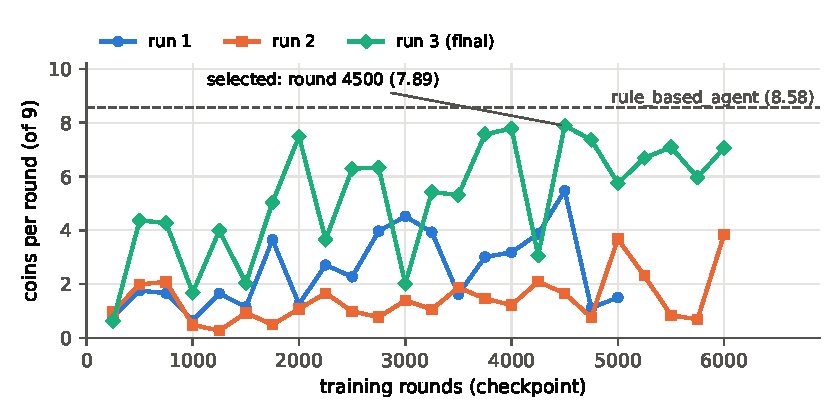
\includegraphics[width=0.85\linewidth]{q_task2_runs.pdf}
\caption{Coins per round of every 250-round checkpoint of the three task-2 runs
(frozen, solo \code{classic}, 150 rounds, seed 42). The dashed line is the
\code{rule\_based\_agent}.}
\label{fig:q-task2}
\end{figure}
 
\begin{table}[htbp]
\centering\small
\caption{Best task-2 checkpoint against the \code{rule\_based\_agent} (solo \code{classic},
150 rounds, seed 42, values per round).}
\label{tab:q-task2}
\begin{tabular}{@{}lrrrrr@{}}
\toprule
Agent & Coins & Crates & Suicides & Bombs & Crates/bomb \\
\midrule
\code{q\_agent} (round 4500) & 7.89 & 109.9 & 0.00 & 45.9 & 2.40 \\
\code{rule\_based\_agent} & 8.58 & 116.6 & 0.00 & 38.1 & 3.07 \\
\bottomrule
\end{tabular}
\end{table}

\subsubsection{Task 3}
\label{sec:q-task3-results}
\authorline{Diana Krasnokutskaya}

All numbers in this section are frozen evaluations on \code{classic} against
\code{peaceful\_agent} + \code{coin\_} \code{collector\_agent}, 100 rounds, seed 42. Margin is our score minus the best opponent's score (Table~\ref{tab:q-task3}).

\begin{table}[htbp]
  \centering\small
  \caption{Q agent on task 3 (frozen, 100 rounds, seed 42).}
  \label{tab:q-task3}
  \begin{tabularx}{\linewidth}{@{}l rrrrrr@{}}
    Model & Score & Kills & Suicides & Coins & Crates & Margin \\
    \midrule
    task-3 checkpoint (\code{model\_3\_diana}), first evaluation & 5.78 & 0.41 & 0.22 & 3.73 & 51.5 & $-1.30$ \\
    best checkpoint of the next run (r2500) & 7.31 & 0.56 & 0.27 & 4.51 & 58.1 & $+0.68$ \\
    after fixes + \code{TRAPPED\_OPPONENT} $=+2$ (r1000) & \textbf{9.78} & \textbf{0.83} & 0.29 & \textbf{5.63} & \textbf{63.6} & $\mathbf{+5.14}$ \\
    \code{model\_3\_diana}, re-evaluated with the final mask & 6.41 & 0.39 & 0.25 & 4.46 & 54.6 & $-0.40$ \\
    \bottomrule
  \end{tabularx}
\end{table}

My checkpoint learned the new behaviour qualitatively: it achieves 0.41 kills per round on average, and it destroys about as many crates as the task-2 agent. It did not yet win, though. With a margin of $-1.30$ it still scored less than the best opponent, usually the coin collector, which competes for the same coins and is not slowed down by bombing crates. The re-evaluation in the last row loads the same weights with the later version of the action mask (voluntary \code{WAIT} banned, a different fallback). The margin improves by 0.9
without any retraining. This shows how much of the agent's behaviour comes from the mask rather than from the learned weights, and it is a caveat for any comparison of Q-agent checkpoints evaluated under different code versions.

The large jump to $+5.14$ came from the next step, which builds on this work: Daniela's fixes for the divergence found in my training log, together with pricing \code{TRAPPED\_OPPONENT} at $+2.0$. Over the 3000 training rounds behind that checkpoint, 82.5\% of rounds ended with our agent ahead of both opponents. The general lesson of task~3 is that for a linear model \textbf{the event that predicts the outcome must carry reward}. \code{BOMBED\_OPPONENT} fires for every bomb near an opponent, most of which the opponent simply walks out of. \code{TRAPPED\_OPPONENT} fires only for bombs the opponent cannot escape, and those are almost always kills. As long as it carried zero reward, the agent had no reason to prefer the bombs that actually work.

To connect task~3 to the tournament, my checkpoint was later also evaluated against three \code{rule\_based\_agent}s ($N = 200$, seed 157): score 3.065, margin $+0.233$ against the mean opponent, strictly first in 23.5\% of rounds, but \textbf{suicide in 61.5\% of rounds}. Hunting weak opponents and surviving a crowded board are different skills. The later task-4 training of the Q agent (section~6.2 \todo{check}) improved exactly this weakness.


\subsubsection{Task 4 and the final model}
\label{sec:q-res-task4}
\authorline{Daniela Ardila}
 
All numbers except Figure~\ref{fig:q-task4-train} are frozen evaluations on
\code{classic}, 100 rounds, seed 42, against one or three \code{rule\_based\_agent}s. The seed fixes only the world, not the random
choices of the \code{rule\_based\_agent}: the same checkpoint measured twice differed by
about 0.1 points, so smaller differences are not meaningful.
 
\paragraph{Reusing the task-3 checkpoint.} Since task 4 used the same 34 features, the
best task-3 checkpoint was the starting point. Figure~\ref{fig:q-task4-train}, the only
training-time measurement here (online, with exploration), shows that training improved
quickly from this start: within the first 1000 rounds, the suicides fell from 0.54
to about 0.38 per round and the kills rose from 0.22 to about 0.35. After that, both
stayed flat for the remaining 5000 rounds, so longer training with the same setup was
unlikely to help.
 
\begin{figure}[htbp]
\centering
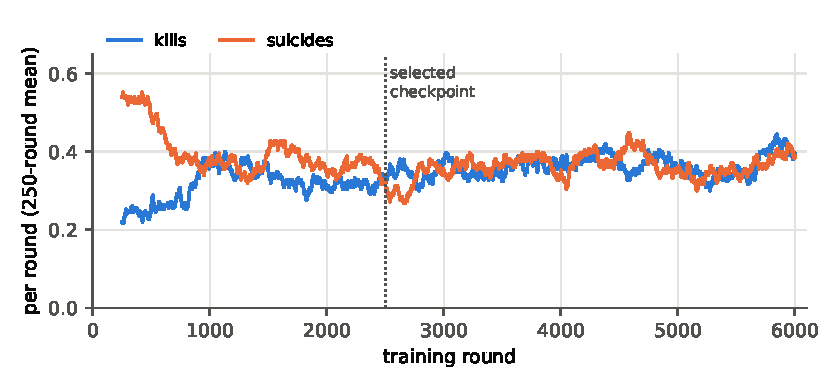
\includegraphics[width=0.85\linewidth]{q_task4_training.pdf}
\caption{Kills and suicides per round during task-4 training against three
\code{rule\_based\_agent}s (online, with exploration; mean over 250 rounds, from
\code{training\_log.csv}).}
\label{fig:q-task4-train}
\end{figure}
 
\paragraph{Selecting the final model.} Figure~\ref{fig:q-task4-ckpt} shows the margin of
every checkpoint against one \code{rule\_based\_agent}. As in task 2, the checkpoints vary
a lot. The best one is in the middle of the run: round 2500 reached $+3.94$, against
$+2.55$ for the starting model, while the last checkpoint reached only $+1.27$. So round
2500 became the final \code{q\_agent}.
 
\begin{figure}[htbp]
\centering
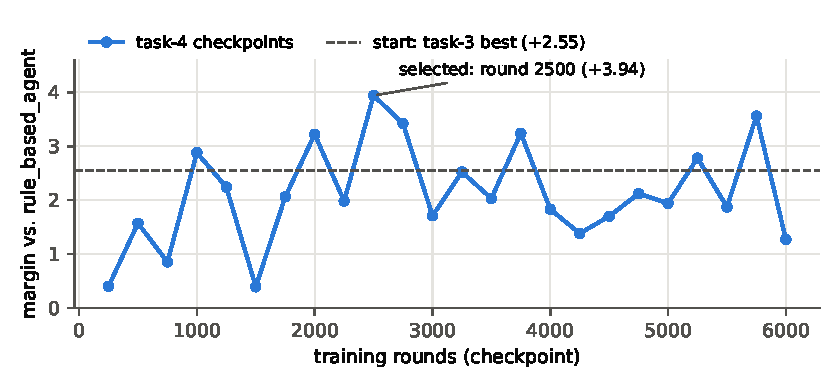
\includegraphics[width=0.85\linewidth]{q_task4_checkpoints.pdf}
\caption{Margin (own score minus opponent's score) of every 250-round task-4 checkpoint
against one \code{rule\_based\_agent} (frozen, 100 rounds, seed 42).}
\label{fig:q-task4-ckpt}
\end{figure}
 
Table~\ref{tab:q-task4} compares the starting model and the final model. Against one
opponent, the final model wins 86\% of the rounds. Against three, it scores almost twice
as much as the best opponent and wins 50\% of the rounds, where an agent as strong as
its opponents would win about 25\%. The largest change is safety: with three opponents,
the suicides fell from 0.55 to 0.22 per round, which was exactly the weakness of the
task-3 agent (Section~\ref{sec:q-task3-results}). With 1000 rounds on a different seed,
Section~\ref{sec:headtohead} confirms this result (score $5.13$, suicides in 25.5\% of
the rounds).
 
\begin{table}[htbp]
\centering\small
\caption{Starting model (best task-3 checkpoint) and final model (task-4 round 2500)
against \code{rule\_based\_agent}s (frozen, \code{classic}, values per round). Win rates
come from 100 single-round games with seeds 0--99.}
\label{tab:q-task4}
\begin{tabular}{@{}llrrrrl@{}}
\toprule
Opponents & Model & Score & Best opp. & Kills & Suicides & Win / tie / loss \\
\midrule
$1\times$ & start & 6.34 & 3.79 & 0.22 & 0.35 & -- \\
          & final & 7.03 & 3.09 & 0.22 & 0.19 & 86\,/\,0\,/\,14\,\% \\
$3\times$ & start & 4.16 & 3.18 & 0.29 & 0.55 & -- \\
          & final & 5.00 & 2.77 & 0.36 & 0.22 & 50\,/\,11\,/\,39\,\% \\
\bottomrule
\end{tabular}
\end{table}

\subsection{The DQN agent}
\label{sec:results_dqn}
\authorline{Luis Maco}

All numbers below are measured frozen (\code{train=False}), with $N \geq 200$ rounds and a
fixed seed list unless noted, and a gate counts as passed only when the whole 95\%
confidence interval clears its threshold.

\subsubsection*{Baselines}

On \code{coin-heaven}, an untrained network acting under an $\varepsilon$-greedy random
policy averages about 18 coins with roughly 145 invalid actions per 400-step round;
\code{rule\_based\_agent} averages 50.0 coins in 125.2 steps with zero invalid actions. On
solo \code{classic}, \code{rule\_based\_agent} averages 8.60 coins with 0\% suicide; in the
four-player tournament shape (three copies of \code{rule\_based\_agent}) it averages a 3.30
mean score with 6.9 invalid actions per round of its own.

\subsubsection*{Gate results}

\begin{table}[h]
\centering
\small
\begin{tabular}{@{}lllll@{}}
\toprule
Task & Gate & Result & Value & $N$ \\
\midrule
1, \code{coin-heaven}    & $\geq$45/50 coins, 0 invalid           & \textbf{PASS} & 46.06 coins, CI [45.5, 46.7] & 200 \\
2, \code{classic} survival & suicide $<2\%$                       & \textbf{PASS} & 0.00\%, 95\% upper 0.38\%     & 1000 \\
2, \code{classic} coins    & $\geq$8/9 coins                      & FAIL          & 2.37 $\pm$ 0.12                & 1000 \\
3, vs \code{peaceful\_agent}   & kill in $\geq$80\% of rounds     & FAIL          & 3.0\% [95\% 2.1, 4.3]         & 1000 \\
3, vs \code{coin\_collector\_agent} & positive margin              & \textbf{PASS} & $+0.89 \pm 0.35$               & 400 \\
4, vs 3$\times$\code{rule\_based\_agent} & mean score strictly above & \textbf{PASS} & $4.961 \pm 0.202$, margin $+2.250 \pm 0.238$ & 1000 \\
\bottomrule
\end{tabular}
\caption{Final candidate (\code{score\_hunt r1250}) against every curriculum gate. Task~4 is
the specification's requirement; Tasks 1--3 are our own curriculum checkpoints.}
\end{table}

Task 1 and Task 4 pass their gates. The selected checkpoint is weaker on the Task 2 solo
test and against the passive opponent in Task 3. An earlier checkpoint
(\code{task4-C-solo-refresh-r1000}, called \emph{C} below) reached $7.70 \pm 0.11$ solo
coins and 76.7\% kill-in-round against \code{peaceful\_agent}, closer to those gates, but
its tournament margin against the weakest of three
\code{rule\_based\_agent}s was only $+0.54 \pm 0.28$, against $+2.18 \pm 0.27$ for the
selected checkpoint. Both pass Task 4, while checkpoint C performs better on the solo and
passive-opponent tests.

\subsubsection*{Measurement and implementation bugs}

Four bugs were identified through measurement.

\begin{enumerate}
\item \textbf{Exploration suicide.} With \code{BOMB} in the random exploration set, the
      agent killed itself within a few steps on \code{coin-heaven}, ending training before
      learning began. We masked \code{BOMB} for Task 1.
\item \textbf{Online policies are not frozen policies.} The same saved weights scored 45
      coins online while the network was updating and 6.2 frozen, a factor of seven. All
      subsequent evaluations therefore use frozen policies.
\item \textbf{Reward shaping paid for idleness.} Covered in Section~\ref{sec:training}: the
      discounted potential term rewarded oscillating near a coin and made collecting a
      distant coin net negative in the worst case.
\item \textbf{Cached \code{next\_state} equalled \code{state}.} A transition cache keyed on
      \code{(round, step)} collided, because the environment increments its step counter
      once, before an agent acts, so the state passed to \code{act()} and its successor
      carried the same key. Instrumentation showed that 800 of 800 sampled transitions had
      \code{next\_state == state} before the fix, and 35.2\% after, consistent with moves
      that leave the agent in the same position. With $s'=s$, the Bellman target becomes
      $r + \gamma \max_a Q(s,a)$ for the same state, preventing value from propagating
      correctly. Wall avoidance was learned almost perfectly, while multi-step coin
      collection was not.
\end{enumerate}

Before the fourth bug was fixed, a six-configuration ablation varying shaping, view,
learning rate, and batch settings placed all configurations between 2.95 and 5.20 frozen
coins with overlapping intervals. This lack of separation led to the transition-cache bug.

\subsubsection*{Specialization under training against \code{rule\_based\_agent}}

A checkpoint trained purely against three \code{rule\_based\_agent}s
(\code{task4-classic-r3250}) passed Task 4 with a $+0.78 \pm 0.25$ margin at $N{=}1000$.
Against the other boards, it lost ground relative to its Task 2 parent: solo
\code{classic} coins fell from 7.51 to 4.34, and kill-in-round against
\code{peaceful\_agent} fell from 69.2\% to 37.7\%, while its self-kill rate did not get
worse (0.60\% $\to$ 0.50\% solo; 42.5\% $\to$ 33.2\% in the crowded game). The bombing
rate also fell, from 47.6 bombs per solo round for the parent to 26.5 for this checkpoint.
The four thousand rounds against \code{rule\_based\_agent}s are consistent with caution
that reduces crate destruction and access to hidden coins in solo play. This suggests
opponent-distribution overfitting on the same seven boards.

The final \code{score\_hunt} checkpoint shows the same pattern. Its bombing rate depends on
the opponent: it is 44.2 bombs per round against three \code{rule\_based\_agent}s, 32.5
against \code{coin\_collector\_agent}, and only 12.5 both solo and against
\code{peaceful\_agent}. This is consistent with its stronger performance on the required
gate and weaker performance on the solo-coin and peaceful-hunting curriculum tests that
earlier checkpoints had passed. Task 4 is the specification's requirement; Tasks 1--3 are
the project's curriculum checkpoints.

\subsubsection*{Hyperparameter sweep and seed sensitivity}

\begin{comment}
\authorline{Diana Krasnokutskaya}

\begin{figure}[htbp]
  \centering
  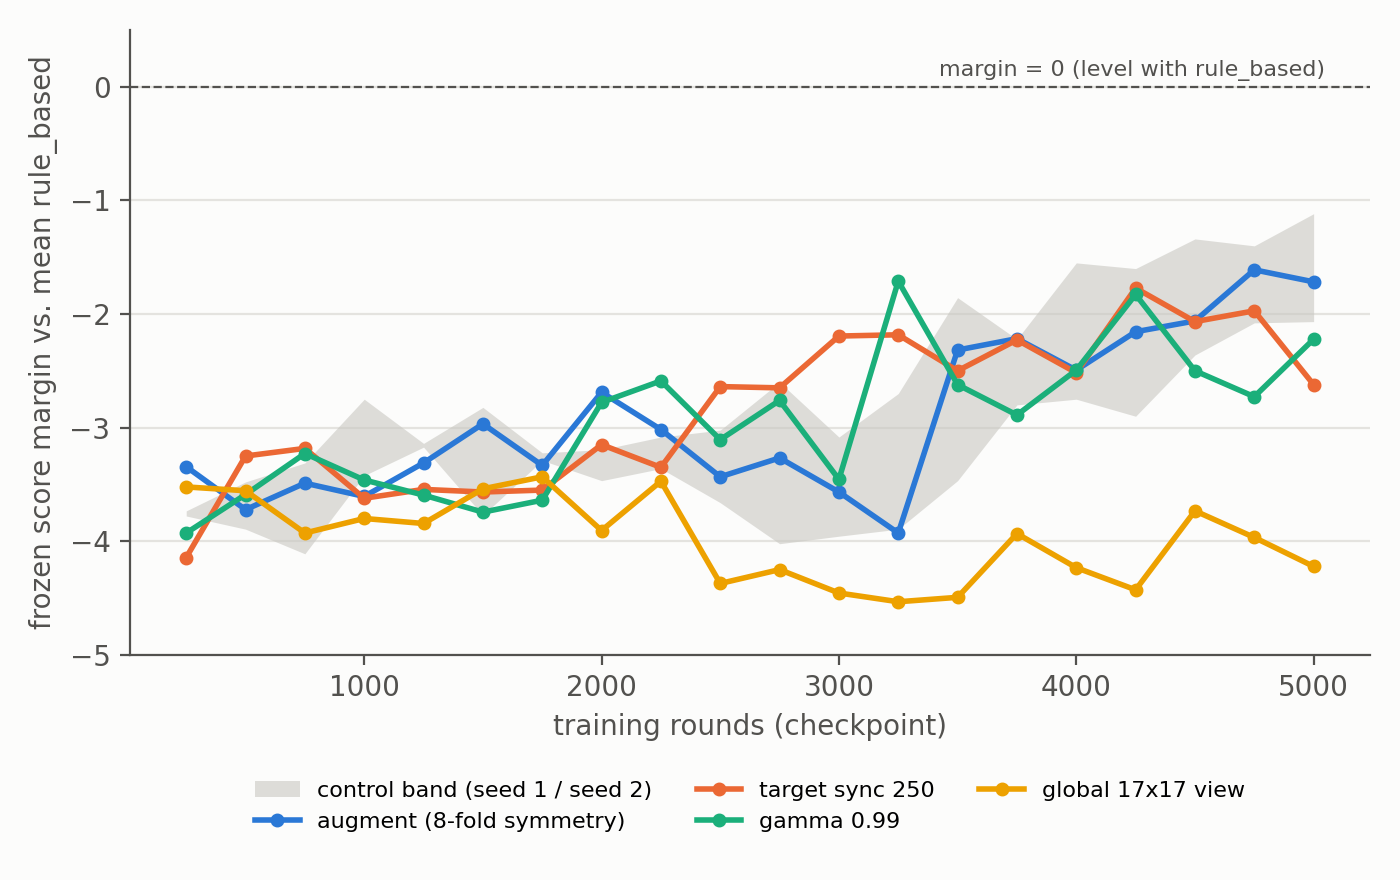
\includegraphics[width=0.9\linewidth]{fig_task4_sweep.png}
  \caption{Frozen margin against the mean \texttt{rule\_based\_agent} for every 250-round
    checkpoint of the task-4 sweep, 60 evaluation rounds each. The grey band spans the two
    control runs, which differ only in their random seed. Values below zero mean the agent
    scores less than the rule-based agents.}
  \label{fig:sweep}
\end{figure}

\begin{table}[htbp]
  \centering\small
  \caption{Task-4 sweep results. Pooled margin is the mean over the last five checkpoints
    (300 rounds).}
  \label{tab:sweep-results}
  \begin{tabular}{@{}l rrrrr@{}}
    \toprule
    Arm & Pooled margin & Best checkpoint & Score & Suicide rate & Kill per round \\
    \midrule
    \code{ctrl_s2}   & $\mathbf{-1.40}$ & $-1.12$ @ r5000 & 1.76 & 31.0\% & 12.0\% \\
    \code{augment}   & $-2.01$ & $-1.61$ @ r4750 & 1.36 & 46.7\% & 12.0\% \\
    \code{target250} & $-2.19$ & $-1.77$ @ r4250 & 1.32 & 46.7\% & 12.0\% \\
    \code{gamma99}   & $-2.35$ & $-1.71$ @ r3250 & 1.14 & 53.0\% & 9.7\% \\
    \code{ctrl_s1}   & $-2.43$ & $-2.07$ @ r5000 & 1.02 & 54.0\% & 10.7\% \\
    \code{global}    & $-4.12$ & $-3.43$ @ r1750 & 0.15 & 6.0\%  & 1.0\% \\
    \bottomrule
  \end{tabular}
\end{table}

\textbf{The two controls are 1.03 margin points apart} (Table~\ref{tab:sweep-results}). They
share every hyperparameter and differ only in the random seed. That spread is the resolution
of the experiment, and almost nothing clears it:
\begin{itemize}
  \item \textbf{$\gamma = 0.99$, target sync 250 and symmetry augmentation all fall inside
        the control band} $[-2.43, -1.40]$. None of them is separated from the control. The
        README's ``raise $\gamma$ for tasks 3 and 4'' is not supported by this measurement.
        The augmentation was the most promising candidate before the sweep, since it has a
        clear mechanistic reason to help an undertrained network (one transition becomes
        eight), and it did not produce a measurable gain either. Our data do not show that
        it is useless. They show that its effect, if any, is smaller than the seed noise at
        this training budget.
  \item \textbf{The global view is the only arm outside the band, and it is clearly worse}:
        1.69 below the \emph{worse} control. On coin-heaven the global view had overtaken
        the egocentric crop after about 1000 rounds, but that result did not transfer. Its
        low suicide rate (6\%) does not mean it learned to handle bombs safely. With a score
        of 0.15 and a kill in 1\% of rounds, it learned mostly to avoid bombing at all. We
        think the likely reason is that on a crowded board the relevant information is local
        (the next bomb, the nearest escape), and a $17\times17$ input dilutes it for a small
        convolutional encoder.
\end{itemize}

The trajectories in Figure~\ref{fig:sweep} show that the egocentric arms were still
improving at round 5000 (for example \code{ctrl_s2}: $-3.17$, $-3.02$, $-2.22$, $-1.12$ at
rounds 1250/2500/3750/5000). The from-scratch agents were therefore probably undertrained
rather than converged. Even so, the best arm ended 1.95 margin points behind the team's
existing curriculum-trained DQN ($+0.55$ margin, 7.8\% suicide at the time), and suicide
rates of 31--54\% show that \textbf{the from-scratch runs never learned bomb safety}. With
the same budget, the curriculum (coins $\rightarrow$ crates $\rightarrow$ score fine-tune)
was far more effective than any of the tested hyperparameters. None of the sweep's models
was a submission candidate.

The control spread also explains an earlier observation. A candidate had been selected on
14.09 because its 40-round evaluation read $+1.42$, and the later $N = 1000$
re-measurement came back at only $+0.55$. Given a seed spread of 1.03 over 300 rounds, the
40-round reading was within the noise, and the correction had to go \emph{down}: the best of
six noisy checkpoints is the one whose noise happened to point up. From then on, every
selected checkpoint was confirmed on a fresh seed with $N = 1000$.
\end{comment}

%???
\begin{figure}[htbp]
  \centering
  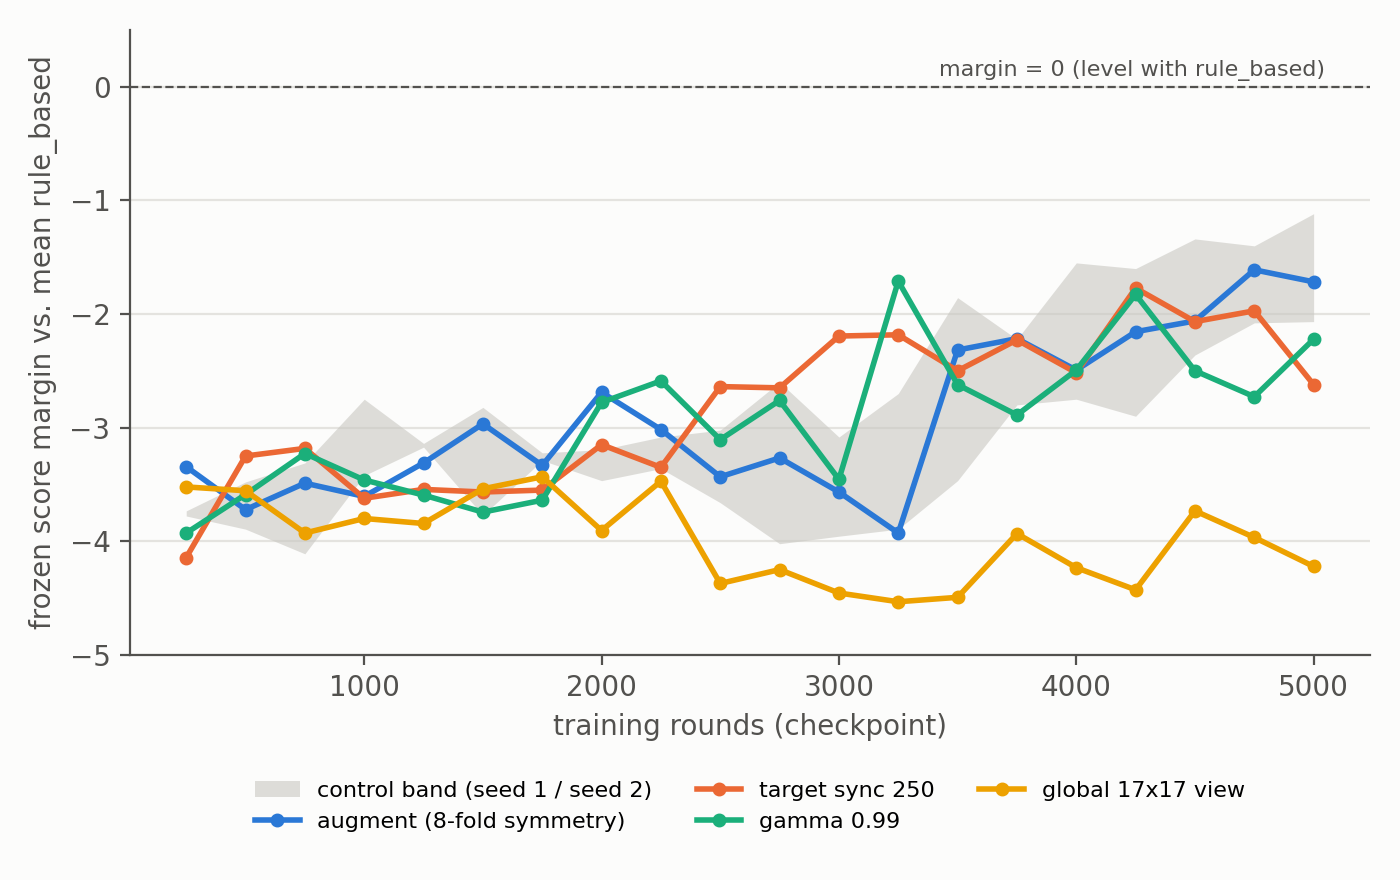
\includegraphics[width=0.9\linewidth]{fig_task4_sweep.png}
  \caption{Frozen margin against the mean \texttt{rule\_based\_agent} for every 250-round
    checkpoint of the task-4 sweep, 60 evaluation rounds each. The grey band spans the two
    control runs, which differ only in their random seed. Values below zero mean the agent
    scores less than the rule-based agents.}
  \label{fig:sweep}
\end{figure}
%???

Six from-scratch configurations were trained for 5000 rounds on \code{classic} against
three \code{rule\_based\_agent}s and ranked over the last five checkpoints (300 pooled
evaluation rounds each). Three changed one hyperparameter relative to control; a fourth used
the global view, and the control was repeated with another seed.

\begin{table}[h]
\centering
\small
\begin{tabular}{@{}lrrr@{}}
\toprule
Configuration & Pooled margin & Suicide & Kill/round \\
\midrule
control (seed A)       & $-1.401$ & 31.0\% & 12.0\% \\
augmentation           & $-2.008$ & 46.7\% & 12.0\% \\
target sync every 250  & $-2.190$ & 46.7\% & 12.0\% \\
discount 0.99          & $-2.354$ & 53.0\% & 9.7\% \\
control (seed B)       & $-2.431$ & 54.0\% & 10.7\% \\
global view            & $-4.117$ & 6.0\%  & 1.0\% \\
\bottomrule
\end{tabular}
\caption{Task-4 hyperparameter sweep, ranked on pooled margin over the last five checkpoints
of a 5000-round from-scratch run.}
\end{table}

The two controls differ by 1.030 margin points.
The augmentation, target-sync, and discount configurations all fall between the two observed
control results, at margins from $-2.354$ to $-2.008$. The global-view configuration falls
outside this range at $-4.117$, 1.686 points below the worse control. This differs from the
Task 1 result, where the global view was the only configuration that kept improving instead
of decaying. Its low 6.0\% suicide rate does not by itself indicate learned bomb safety:
the same configuration scored 0.15 and killed an opponent in only 1\% of rounds.

No from-scratch run closed the roughly two-point gap to the incumbent within budget. The
runs had not clearly flattened by round 5000; the control's margin moved
$-3.17 \to -3.02 \to -2.22 \to -1.12$ across the run. The results therefore do not
establish that the tested factors are unimportant with longer training. We stopped after
the sweep because no tested configuration had matched the already-confirmed incumbent
within the available budget.

\subsubsection*{Selection}

\code{score\_hunt r1250} was chosen as the final DQN tournament candidate on Task 4, the
specification's required gate. It was shortlisted from a 40-round-per-checkpoint curve,
confirmed at $N{=}200$ on an unseen seed, and re-confirmed at $N{=}1000$ on a second unseen
seed. Its three individual paired margins against the three
\code{rule\_based\_agent}s are $+2.290 \pm 0.265$, $+2.281 \pm 0.271$, and
$+2.178 \pm 0.267$; every 95\% lower bound is above $+1.9$. Checkpoint \emph{C} also
passes Task 4 with a smaller positive margin and performs better on the solo and
passive-opponent tests reported above, but has a higher crowded-room suicide rate
(32.5\% against 10.9\%).

\subsubsection*{Controlled comparison with the feature-based agent}

Using the shared frozen comparison protocol (\code{tools/compare\_team\_agents.py}), both
agents were evaluated separately against the same seeded three-\code{rule\_based\_agent}
opponents at $N{=}200$ on seed 157. The DQN scored $4.615 \pm 0.385$ against the
feature-based agent's $3.065 \pm 0.320$, with a mean margin over the three opponents of
$+1.858 \pm 0.465$ against $+0.233 \pm 0.403$, and was strictly first in 43.0\% of rounds
against 23.5\%. Under this protocol, the DQN passed the required Task 4 gate and the
feature-based checkpoint tested at that time did not.

The DQN's Task 4 result was later confirmed at $N{=}1000$ on a separate seed, as reported
above. The feature-based agent was not re-evaluated at that sample size within the project
timeline, so the tournament-entry decision used the $N{=}200$ controlled comparison. The
tested feature-based checkpoint was the checkpoint available for comparison at the time;
it was not independently verified as the owner's final intended submission.

%---------------------------------------------------------------??????

\subsection{Head-to-head: Q agent vs.\ DQN on the same board}
\label{sec:headtohead}
\authorline{Diana Krasnokutskaya}

On 16.09 the team compared the two agents by evaluating each one \textbf{separately}
against three \code{rule\_based\_agent}s. The DQN (\code{score\_hunt} r1250) scored 4.615 and
the Q agent 3.065, and the DQN was selected as the tournament agent. I checked this
comparison in two ways before the code deadline.

\paragraph{Which Q model was measured?}
The comparison script had loaded the Q checkpoint from my commit \code{c0f36d7}, a copy
placed into the DQN branch for a meeting on 15.09, not the current Q model (\code{f00baeb},
after task-4 training). Replaying \code{c0f36d7} in the identical protocol ($N = 200$, seed
157) reproduced every metric of the 16.09 run to three decimals, on two machines and two
operating systems. This is possible because the seed fixes both the world's and the agents'
random number generators and the frozen Q policy is a deterministic masked argmax. The 16.09
measurement was correct, but its ``Q agent'' row described a model three versions old.

\paragraph{Current models, same protocol.}
Table~\ref{tab:seed223} shows the current Q model re-measured on the same seed as the DQN's
own $N = 1000$ confirmation (seed 223, three \code{rule\_based\_agent}s).

\begin{table}[htbp]
  \centering\small
  \caption{Each agent separately against three \texttt{rule\_based\_agent}s ($N = 1000$, seed
    223). $\pm$ is the 95\% confidence interval half-width.}
  \label{tab:seed223}
  \begin{tabular}{@{}l rrr@{}}
    \toprule
    Agent & Score & Margin vs.\ mean opponent & Suicide rate \\
    \midrule
    DQN \code{score\_hunt} r1250 & $4.961 \pm 0.202$ & $+2.250 \pm 0.238$ & \textbf{10.9\%} \\
    Q agent \code{f00baeb} & $\mathbf{5.126 \pm 0.213}$ & $\mathbf{+2.482 \pm 0.250}$ & 25.5\% \\
    \bottomrule
  \end{tabular}
\end{table}

Both agents clearly pass the task-4 gate. The DQN's lead is gone, although the intervals
overlap. The DQN is still the safer policy, suiciding about half as often.

\paragraph{Paired comparison on one board.}
Evaluating both agents separately compares them against different opponents and different
boards. The tournament puts them on the same board, where they compete for the same coins
and can kill each other. So I ran both team agents plus two \code{rule\_based\_agent}s
together (four players, \code{classic}, training off, $N = 1000$, seed 409). Every round is
then a paired observation with identical opponents, crates and coins
(Figure~\ref{fig:h2h}, Table~\ref{tab:h2h}).

\begin{figure}[htbp]
  \centering
  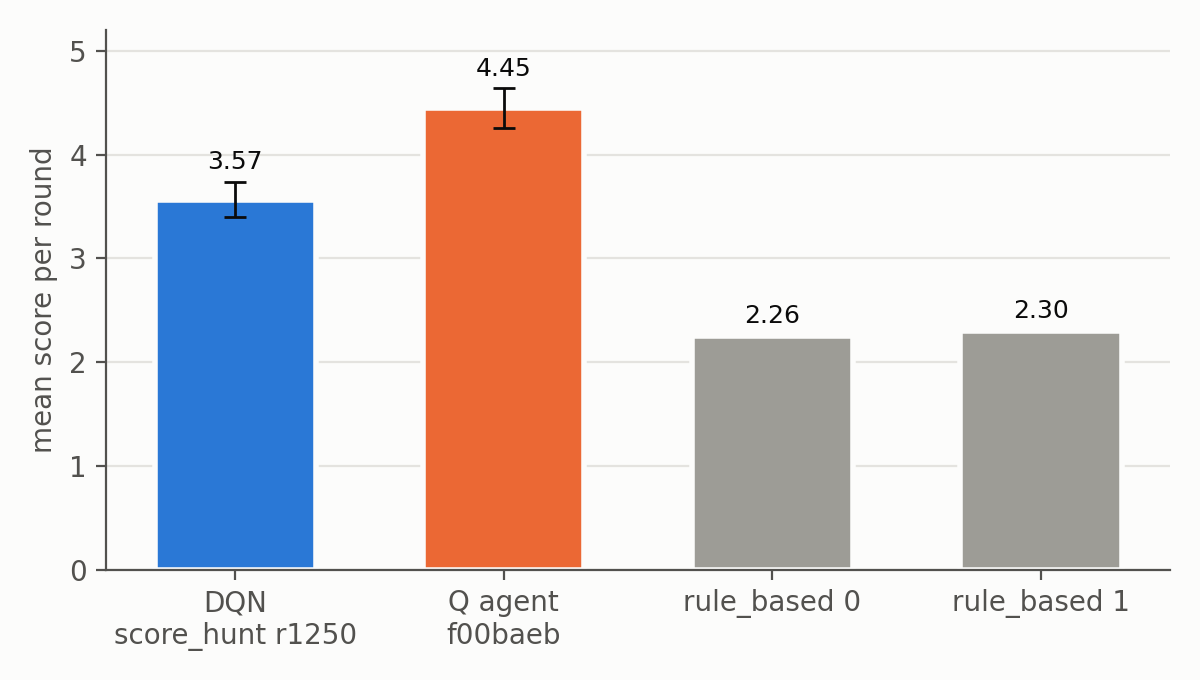
\includegraphics[width=0.72\linewidth]{fig_headtohead.png}
  \caption{Mean score per round over 1000 four-player rounds (seed 409); error bars are
    95\% confidence intervals.}
  \label{fig:h2h}
\end{figure}

\begin{table}[htbp]
  \centering\small
  \caption{Head-to-head on one board: both team agents and two \texttt{rule\_based\_agent}s
    ($N = 1000$, seed 409).}
  \label{tab:h2h}
  \begin{tabular}{@{}l rrrr@{}}
    \toprule
    Metric & DQN \code{score\_hunt} r1250 & Q agent \code{f00baeb} & \code{rule\_based} 0 & \code{rule\_based} 1 \\
    \midrule
    score           & $3.567 \pm 0.17$ & $\mathbf{4.448 \pm 0.19}$ & 2.257 & 2.304 \\
    coins           & 2.407 & \textbf{2.988} & 1.787 & 1.789 \\
    kills           & 0.232 & \textbf{0.292} & 0.094 & 0.103 \\
    suicide rate    & 29.4\% & \textbf{22.2\%} & 39.4\% & 39.0\% \\
    invalid actions & \textbf{0.859} & 1.564 & 5.194 & 5.269 \\
    \bottomrule
  \end{tabular}
\end{table}

The paired margin DQN $-$ Q is $\mathbf{-0.881 \pm 0.286}$ (95\% interval
$[-1.167, -0.595]$), so the whole interval lies below zero. The Q agent finished ahead in
52.5\% of rounds, the DQN in 37.2\%, and 10.3\% were ties. Both still beat the rule-based
agents (DQN $+1.286 \pm 0.207$, Q $+2.167 \pm 0.226$ against their mean). A pilot with
$N = 200$ on a different seed (157) had given $-0.870 \pm 0.607$. The $N = 1000$
confirmation moved the point estimate by 0.011 and narrowed the interval by a factor of two,
which is good evidence that the result is not a seed artefact. A 1-vs-1 of the two agents
alone ($N = 200$) gives $-2.690 \pm 0.576$ and 70.5\% of rounds to the Q agent. That setting
has more crates and coins per player and no third-party bombs, so we report it only as
context, not as a tournament claim.

Notably, the DQN's suicide rate almost triples (10.9\% $\rightarrow$ 29.4\%) when the Q
agent replaces one rule-based agent. The Q agent apparently creates situations the DQN,
fine-tuned only against rule-based opponents, has never seen. This matches the DQN audit in
section~6.2 \todo{check}: the \code{score\_hunt} checkpoint is a specialist for exactly one
opponent type.

\paragraph{Consequence.}
The DQN had been selected on the basis of the 16.09 comparison, and that basis no longer
holds. The Q agent is ahead or level in every configuration we measured, and it is ahead
with a separated confidence interval in the only configuration shaped like the tournament.
Two caveats remain. None of our configurations \emph{is} the tournament, where the opponents
are other teams' agents. And the DQN's lower suicide rate in the solo protocol might matter
against opponents that punish mistakes harder than \code{rule\_based\_agent} does. Since the
tournament ranks by score, we submitted the \textbf{\code{q\_agent}} \todo{confirm final
choice: \code{q\_agent} or \code{dqn\_agent}} as our tournament agent.

To make this comparison reproducible, I merged both agent branches into \code{master}, so
the comparison is a single command:
\begin{lstlisting}
python tools/evaluate3.py --agents dqn_agent q_agent rule_based_agent 
rule_based_agent \ --scenario classic --n-rounds 1000 --seed 409
\end{lstlisting}
The merge also removed the stale \code{c0f36d7} copy of the Q agent from the DQN branch,
which had caused the mix-up in the first place. The raw per-round results of all five runs
are stored under \code{experiments/runs/} with the prefix \code{20260917-}.

% ============================================================
\section{Conclusion}
% ============================================================
\authorline{Diana Krasnokutskaya}

We trained two structurally different reinforcement learning agents for Bomberman: a linear Q-learning agent over 34 hand-engineered features, and a Double DQN that learns its own features from a six-channel image of the board. Both went through the same curriculum (coins, crates, weak opponents, \code{rule\_based\_agent}), and both pass the requirement for the tournament: in frozen play on \code{classic} against three \code{rule\_based\_agent}s, each scores clearly more than its opponents (margins of $+2.48$ and $+2.25$ over 1000 rounds). On a shared board, however, the Q agent beats the DQN by 0.88 points per round, with a confidence interval that excludes zero, and it finishes ahead in 52.5\% versus 37.2\% of rounds.

The main findings of the project, as I see them, are:
\begin{enumerate}
  \item \textbf{Domain knowledge was worth more than representational power at our budget.} The linear agent's features already encode path distances, blast timing and escape routes, so its learning problem is small. The DQN has to discover all of this from image-like input. In three weeks on single CPU threads it learned a safer but less productive policy, and the from-scratch sweep showed that it does not learn bomb safety at all without the curriculum.
  \item \textbf{Safety is structural, not only learned.} Both agents rely on an action mask that removes provably suicidal actions, and for the Q agent, changing only the mask moved a checkpoint's margin by 0.9 without retraining. Getting the blast and escape model \emph{exactly} right, down to the step at which an explosion is lethal, was a prerequisite for everything else.
  \item \textbf{The reward must pay for the event that predicts success.} For the Q agent the most effective single change was rewarding bombs an opponent cannot escape, rather than any bomb near an opponent.
  \item \textbf{Measurement is the hard part.} Two runs that differed only in their seed ended 1.03 margin points apart, and this was larger than the effect of any hyperparameter we tested. Selecting the best of several short evaluations inflated a candidate's value from $+1.42$ to a true $+0.55$. Evaluating two agents separately instead of on the same board, and with a stale checkpoint, led to the wrong tournament choice until we re-checked. Frozen evaluation, fixed seeds, confidence intervals, a second control run, confirmation on a fresh seed with $N = 1000$, and paired comparisons turned out to matter more than any single modelling trick.
\end{enumerate}

\paragraph{If we had more time,} we would work on the following:
\begin{itemize}
  \item \textbf{Train against more varied opponents, including self-play.} A pool of past checkpoints of both agents and other teams' shared agents would address the DQN's over-specialisation.
  \item \textbf{Give the DQN the Q agent's knowledge}, for example the engineered danger and escape features as extra input channels, or a warm start by imitating the Q agent before RL fine-tuning.
  \item \textbf{Reduce the Q agent's remaining suicides} (22\% in the head-to-head). The escape check assumes that opponents stand still; predicting where they can move within the fuse time would close most of the remaining gaps.
  \item \textbf{Run longer DQN experiments with at least three seeds per configuration}, since the sweep's curves were still rising at 5000 rounds and one seed per arm is below the observed noise level.
\end{itemize}

\paragraph{For next year's game setup,} we would suggest:
\begin{itemize}
  \item Report per-agent statistics in the round summary. The framework currently sums coins, kills and suicides over all agents, so from task~3 on every team has to write its own evaluation script.
  \item Document exactly at which steps a bomb makes a tile lethal. We had to reverse-engineer this from \code{environment.do\_step}, and an off-by-one error there directly causes suicides.
  \item Provide a reference evaluation script with seeds and confidence intervals, which would make results comparable across teams.
\end{itemize}

\begin{comment}
% ============================================================
\section*{Work distribution}
% ============================================================
\begin{table}[h]
\centering
\small
\begin{tabular}{@{}lll@{}}
\toprule
WP & Topic & Lead \\
\midrule
WP1  & Data pipeline and preprocessing        & D.~Krasnokutskaya \\
WP2a & Dense autoencoder                       & D.~Krasnokutskaya \\
WP2b & Convolutional autoencoder               & J.~Mutluer \\
WP3  & Optimizers, training loop, metrics      & J.~Mutluer \\
WP4  & Latent-space and robustness analysis    & D.~Krasnokutskaya \\
WP5  & Poster and report                       & both \\
\bottomrule
\end{tabular}
\end{table}
\end{comment}

% ============================================================
\begin{thebibliography}{99}
% ============================================================
\bibitem{mnih2015} V.~Mnih, K.~Kavukcuoglu, D.~Silver, et al.
  \emph{Human-level control through deep reinforcement learning.}
  Nature, 518(7540):529--533, 2015.
\bibitem{vanhasselt2016} H.~van Hasselt, A.~Guez, and D.~Silver.
  \emph{Deep Reinforcement Learning with Double Q-learning.}
  Proc.\ AAAI Conference on Artificial Intelligence, 2016.
\bibitem{ng1999} A.~Y.~Ng, D.~Harada, and S.~Russell.
  \emph{Policy Invariance Under Reward Transformations: Theory and Application to Reward
  Shaping.} Proc.\ 16th International Conference on Machine Learning (ICML), 1999.
\bibitem{pardo2018} F.~Pardo, A.~Tavakoli, V.~Levdik, and P.~Kormushev.
  \emph{Time Limits in Reinforcement Learning.}
  Proc.\ 35th International Conference on Machine Learning (ICML), 2018.
% Add citations backing the Background and Q-learning sections here.
\bibitem{koethe2026mle} U.~K\"othe.
  \emph{Machine Learning Essentials: Reinforcement Learning, Parts 1 and 2.}
  Lecture, Heidelberg University, 14--16 July 2026.
\bibitem{sutton2018} R.~S.~Sutton and A.~G.~Barto.
  \emph{Reinforcement Learning: An Introduction.}
  2nd edition, MIT Press, 2018.
\bibitem{sutton1988} R.~S.~Sutton.
  \emph{Learning to Predict by the Methods of Temporal Differences.}
  Machine Learning, 3(1):9--44, 1988.
\bibitem{watkins1992} C.~J.~C.~H.~Watkins and P.~Dayan.
  \emph{Q-learning.}
  Machine Learning, 8(3--4):279--292, 1992.
\bibitem{rummery1994} G.~A.~Rummery and M.~Niranjan.
  \emph{On-line Q-learning Using Connectionist Systems.}
  Technical Report CUED/F-INFENG/TR~166, Cambridge University, 1994.
\bibitem{singh2000} S.~Singh, T.~Jaakkola, M.~L.~Littman, and C.~Szepesv\'ari.
  \emph{Convergence Results for Single-Step On-Policy Reinforcement-Learning Algorithms.}
  Machine Learning, 38(3):287--308, 2000.
\bibitem{vanhasselt2018} H.~van Hasselt, Y.~Doron, F.~Strub, et al.
  \emph{Deep Reinforcement Learning and the Deadly Triad.}
  arXiv:1812.02648, 2018.
\bibitem{schulman2017} J.~Schulman, F.~Wolski, P.~Dhariwal, A.~Radford, and O.~Klimov.
  \emph{Proximal Policy Optimization Algorithms.}
  arXiv:1707.06347, 2017.
\bibitem{browne2012} C.~B.~Browne, E.~Powley, D.~Whitehouse, et al.
  \emph{A Survey of Monte Carlo Tree Search Methods.}
  IEEE Transactions on Computational Intelligence and AI in Games, 4(1):1--43, 2012.
\bibitem{ross2011} S.~Ross, G.~J.~Gordon, and J.~A.~Bagnell.
  \emph{A Reduction of Imitation Learning and Structured Prediction to No-Regret Online Learning.}
  Proc.\ 14th International Conference on Artificial Intelligence and Statistics (AISTATS), 2011.
 

\end{thebibliography}



\end{document}

